\subsection{The cross section of the $d(K^-, n)"\pi^{\mp}\Sigma^{\pm}$}

The Monte Calro simulation of $d(K^-, n)"\pi^{\mp}\Sigma^{\pm}$ reaction was performed to decompose each modes.
The simulation data was used to estimate the acceptance as function of $d(K^-, n)"\pi^{\mp}\Sigma^{\pm}"$ to adopt same analysis procedure,
so this acceptance includes $d(K^-, n \pi^+ \pi^-)"n"$ selection efficeincy , rejection ratio of $\Sigma^{\pm}_{forward}$ and $K^0$ and so on.
Fig\ref{fig:charge_mode_acc} shows these acceptances.
Spectra of the $d(K^-, n)"\pi^{\mp}\Sigma^{\pm}"$ was converted to the cross section these acceptances and conversion factor which was summrized at Table\ref{tab:KN_scale}.
Obtained cross sections are represented at Fig\ref{fig:Charge_CS}.
Inner box indicates statical error of the $d(K^-, n)"\pi^{\mp}\Sigma^{\pm}"$ events, outer box indicates errors convolved fitting error
and error bars indicates error includeing all error which is statical error, fitting error and conversion factor error.

\begin{figure}[htbp]
  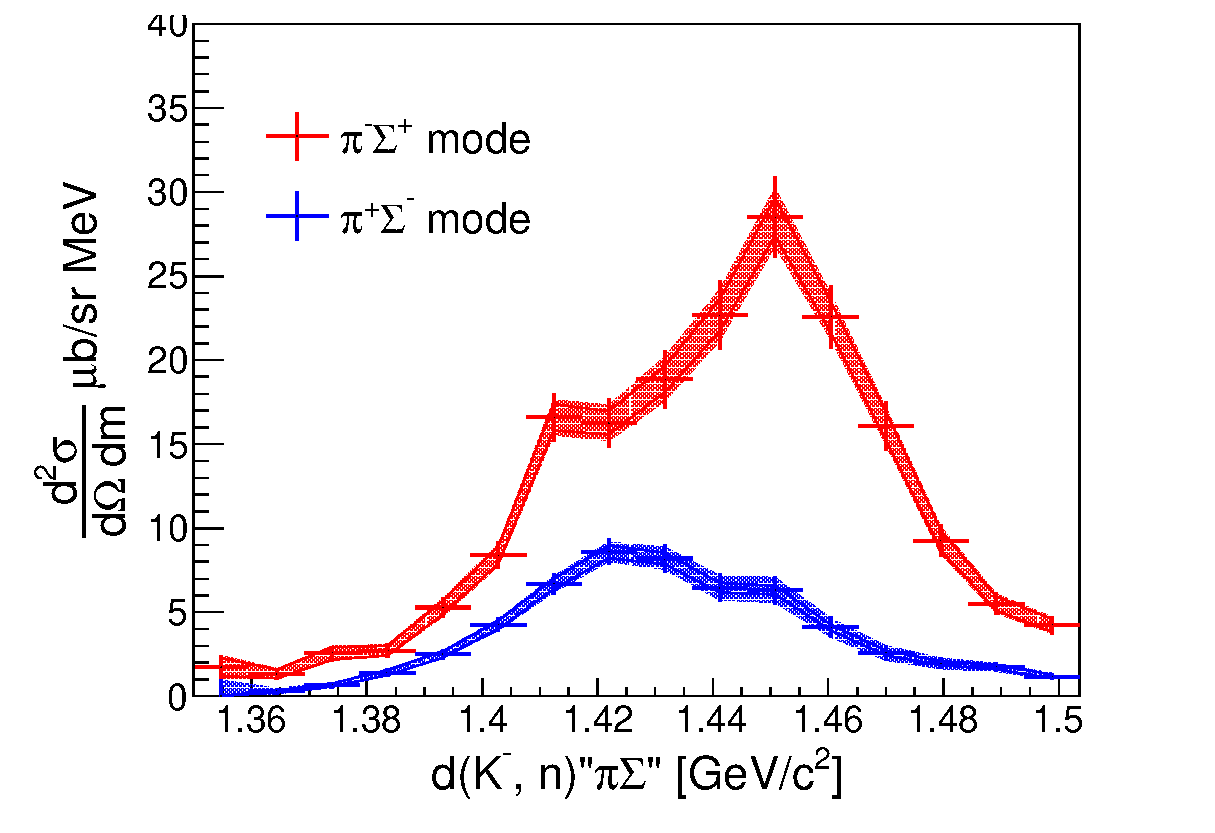
\includegraphics[width=12cm]{../pic/Dron/charge_CS_wts.eps}
  \caption{
    This figure shows cross sections os $d(K^-, n)"\pi^{\mp}\Sigma^{\pm}"$ which convolve $K^0$ 2step effect discribed at Sec\label{sec:K0_2step}.
  }
  \label{fig:Charge_CS}
\end{figure}

